\ofsection{Game Master}
%
\ofquote{"Tough... Don't blame us. Blame yourself or God."\\}{Delita}\\\\
%
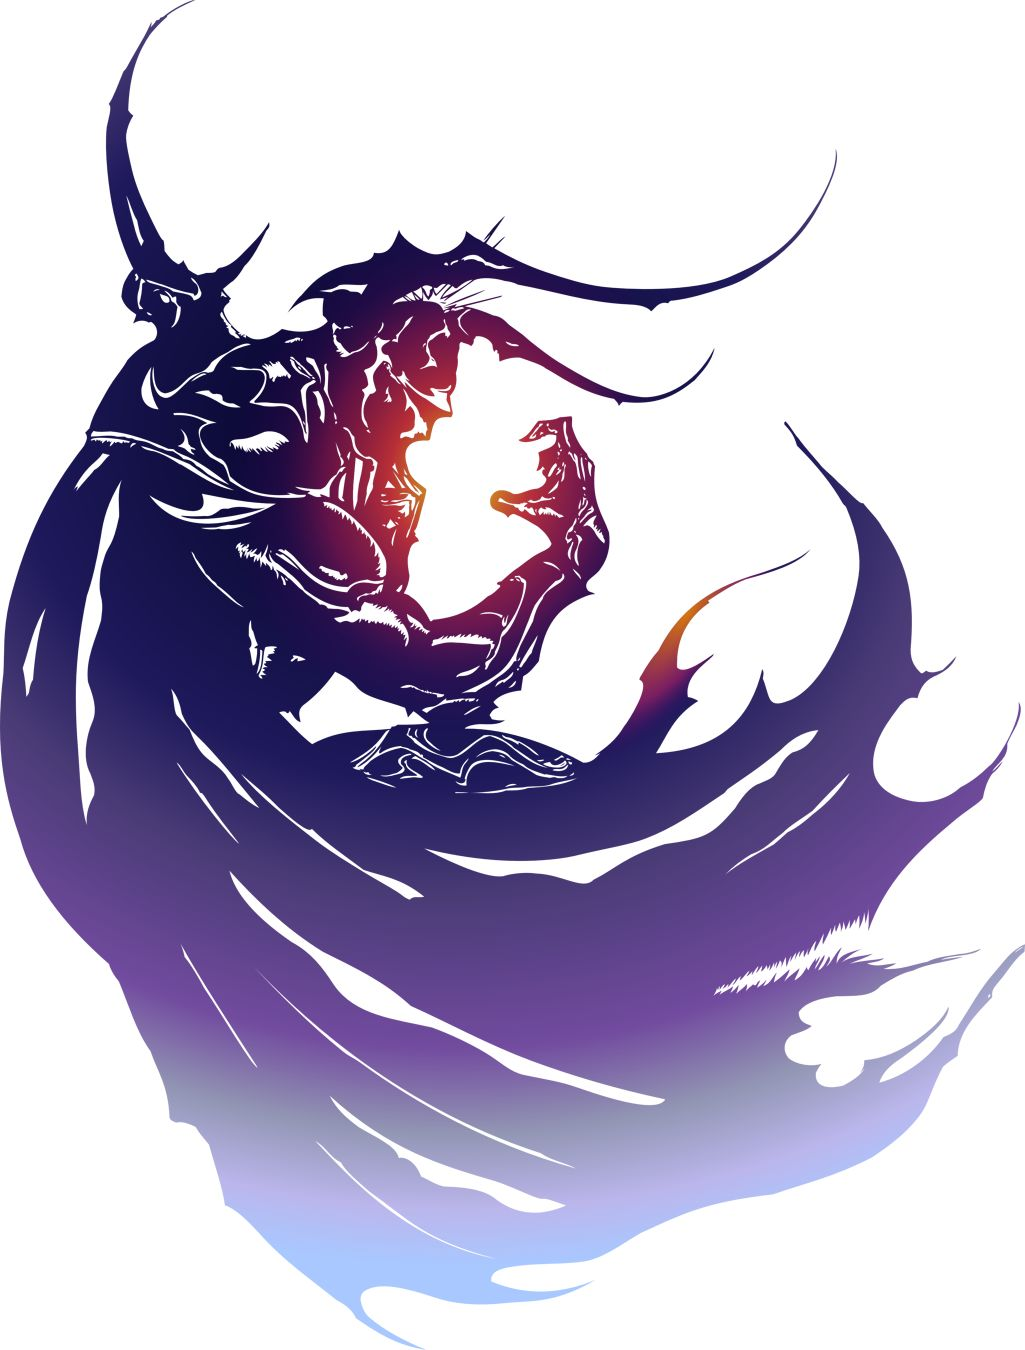
\includegraphics[width=\columnwidth]{./art/images/ff4.jpg}
%
\vfill
%
Compared to the players, who play the game from the perspective of the protagonists, the \accf{Game Master} has a different role.
He creates the world and setting of the adventure and takes the role of all non-player characters.
Furthermore, the GM describes the environment and narrates the outcomes of most actions. 
Unlike the players, the GM is not bound by strict rules and may make his own rulings when necessary.
There is no single way to be a successful GM and we encourage you adopt a style that is enjoyable for both you and the players.
%
\vfill
%
Accordingly, this chapter does not focus on presenting rules or advice.
Instead, it is a collection of modular \accf{supplements}, that you can either use directly or regard as examples for creating your own content.
These supplements not only to give a glimpse into the various aspects of game mastering, but also show some of the different directions that you can take with Omega Fantasy. 
The present modules can be broadly split into two categories: \accf{prepared content} and \accf{rule changes}.
The former provide you with world building blocks such as adventures, settings and monsters that are self-contained and extensible.
The latter present you examples to customize the rules to your preferences.
While the prepared content is well suited for beginners, we recommend to consider rule changes once you have gathered some experience with Omega Fantasy.
All available supplements are listed in the following, together with a short synopsis for each one.
%
\newpage
%
\accf{Bestiary:} this section discusses guidelines for creating interesting monsters and combat encounters.
Furthermore, it includes a large collection of prepared enemies that you can either directly use for you game or regard as examples for creating your own ones.
%
\vfill
%
\accf{Chaos in Cornelia:} a short adventure in which the party has to save a kidnapped princess. 
Highly recommended for beginners and provides an easy entry into Omega Fantasy.
Contains diverse content covering different aspects of adventuring, such as combat, roleplaying and exploration.
%
\vfill
%
\accf{Tomb of Raithwall:} a short adventure in which the party has to recover an ancient artifact from a dangerous tomb.
Focused on exploring a challenging environment where traps and adversaries may lurk around every corner. 
%
\vfill
%
\accf{Maria \& Draco:} a single-session adventure in which the party has to ensure the success of an opera performance.
Encourages a more light-hearted narrative with a focus on interesting roleplaying moments.
%
\vfill
%
\accf{Siege of Dollet:} a single-session adventure in which the party has to pass a practical test to join an elite mercenary force.
Focuses on creating an action packed narrative with multiple combat encounters.
%
\vfill
%
\accf{Gold Saucer:} an amusement park where the party can blow off steam and win rare prizes. 
This one is more loosely structured and focuses on recreating the various games in the park, which can serve you as an example on how to create non-combat competitions.  
%
\vfill
%
\accf{Ivalice Worldbook:} a very detailed document focused on fleshing out the world of Ivalice, including its history and geography.
This helps you to create various adventures in this world, but it can also serve as an example of how to create a detailed setting.
%
\vfill
%
\accf{Optional Rules:} minor rule changes and additions that help you to customize the feeling of the game.
%
\vfill
%
\accf{Races:} rules and examples for incorporating different humanoid races in your world. 
This provides additional character creation options for players, but can also help you to create a more interesting game world.
%
\vfill
%
\accf{Chocobos:} rules for incorporating bird-like creatures called Chocobos as full-fledged party members.
Players can raise Chocobos, use them as mounts and fight alongside them in combat.
%
\vfill
%
\accf{Triple Triad:} rules for a fun card game, allowing the party to collect and play cards.
Well suited if you are looking quick and simple side-activity for the party.
%
\vfill
%
\accf{Blitzball:} rules for a fun team-based sports game similar to water polo.
Well suited if you are looking for a more elaborate side-activity for the party.
%
\vfill
%
\accf{Filled Character Sheets:} sheets for Level~1 characters that you or the players can directly use or regard as examples for creating your own.
%
\clearpage